\documentclass{article}
\usepackage{cleveref}
\usepackage[margin=1in]{geometry}
\usepackage{graphicx}
\graphicspath{{images/}}

\author{Collin Walther \and Phi Lam}
\title{User Guide for the SCU Course Equivalency System}

\begin{document}
\maketitle

\section{Introduction}
The SCU Course Equivalency System is a web-based solution which allows SCU
faculty members to easily keep track of and refer to course equivalencies.
Using this system, faculty members can keep track of which courses from other
universities count for which courses inside of SCU, greatly improving the speed
at which professors can approve transfer credit from other schools.

\section{Public Functionality}
\par The system uses a web-based interface. To access it, open a web browser
and navigate to \\students.engr.scu.edu/\textasciitilde cwalther/SoftwareEngineeringProject.php.
This is the home page, and it will look like the
image shown in \cref{fig:homepage}.

\begin{figure}[h]
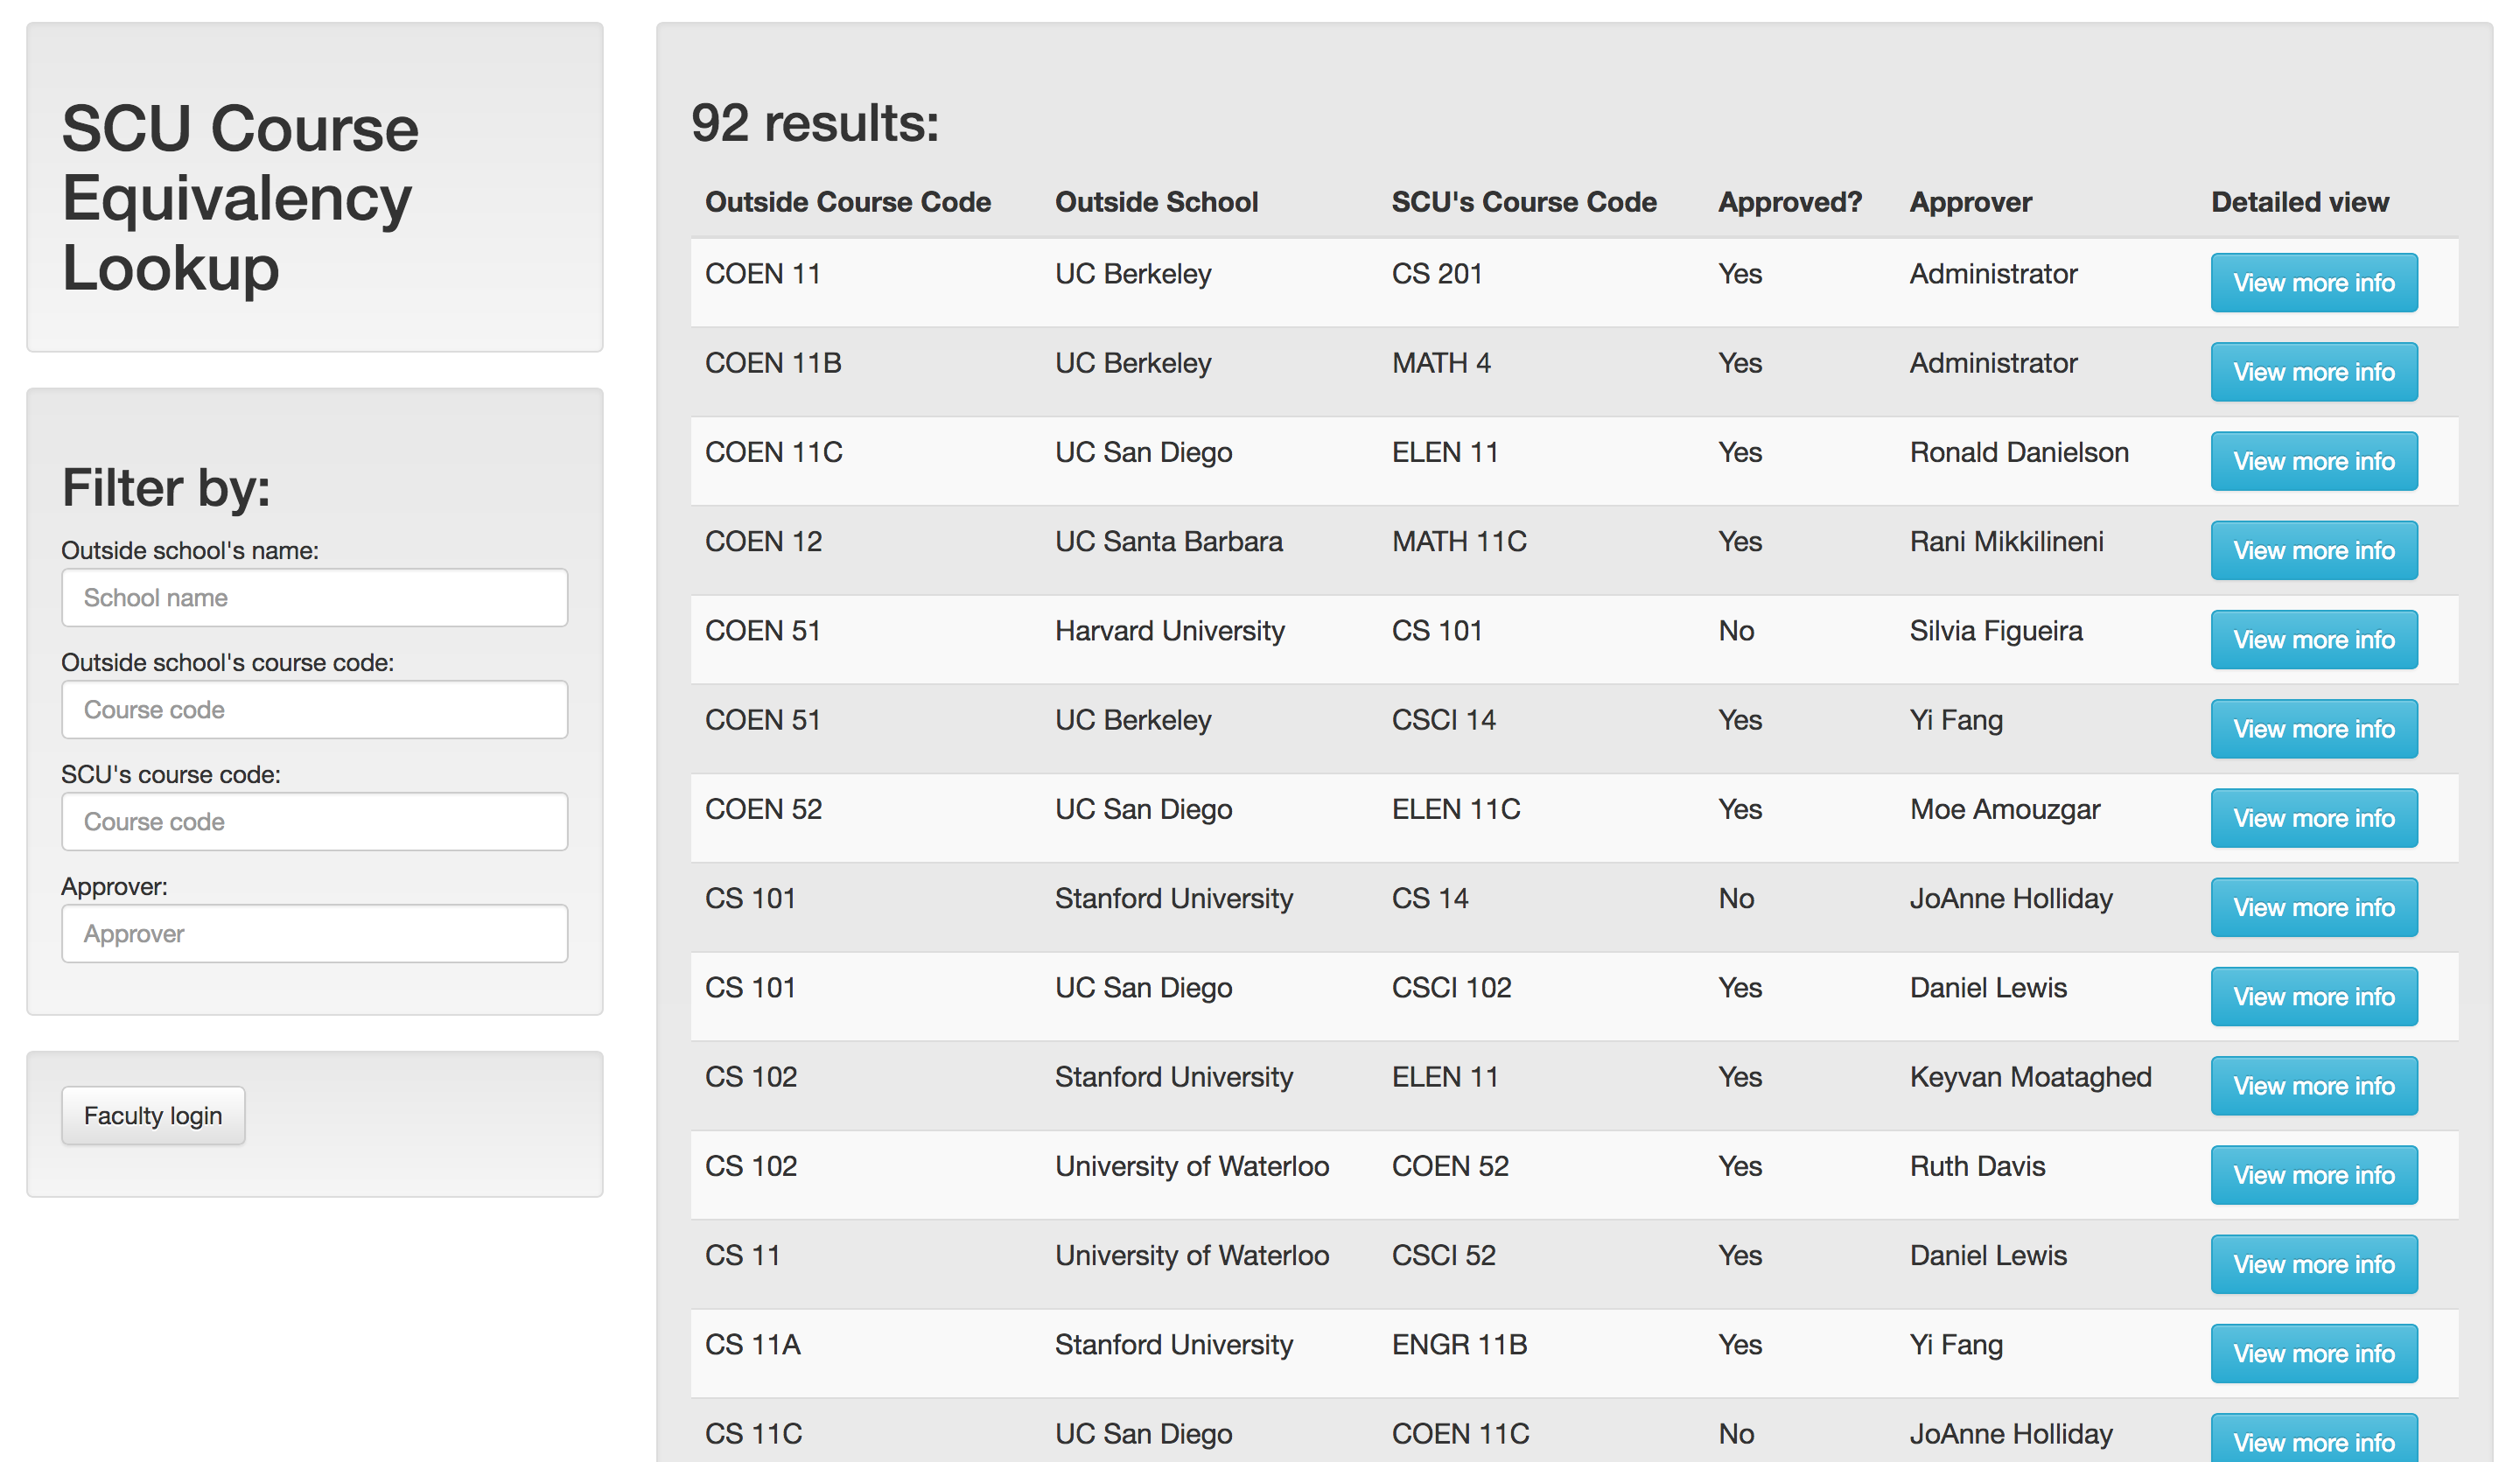
\includegraphics[width=15cm]{homepage}
\centering
\caption{Home page}
\label{fig:homepage}
\end{figure}

\par There are a few elements of the system that are noticeable here. On the
left side of the screen are the title of the system, the search fields, and
the faculty login button. On the right side of the screen are all of the
course equivalencies that match the current search queries.

\par To search for a particular course equivalency determination, you can fill
out the various search fields (``Outside school's name'', ``Outside school's course
code'', ``SCU's course code'', and ``Approver'') located in the box on the left
headed by ``Filter by''. When you do this, the search results on the right side
of the screen will be refined to only include results matching the search terms.

\par If you would like to view more info about any equivalency, such as the
notes added by the instructor when he/she created the equivalency, then you may
click the blue ``View more info'' button to the right of the equivalency. This
will redirect you to another page, shown in \cref{fig:detailedview}. On this page, you may view
notes added by the instructor about the equivalency. To return to the home
page, click the ``Back to home'' link.

\begin{figure}[h]
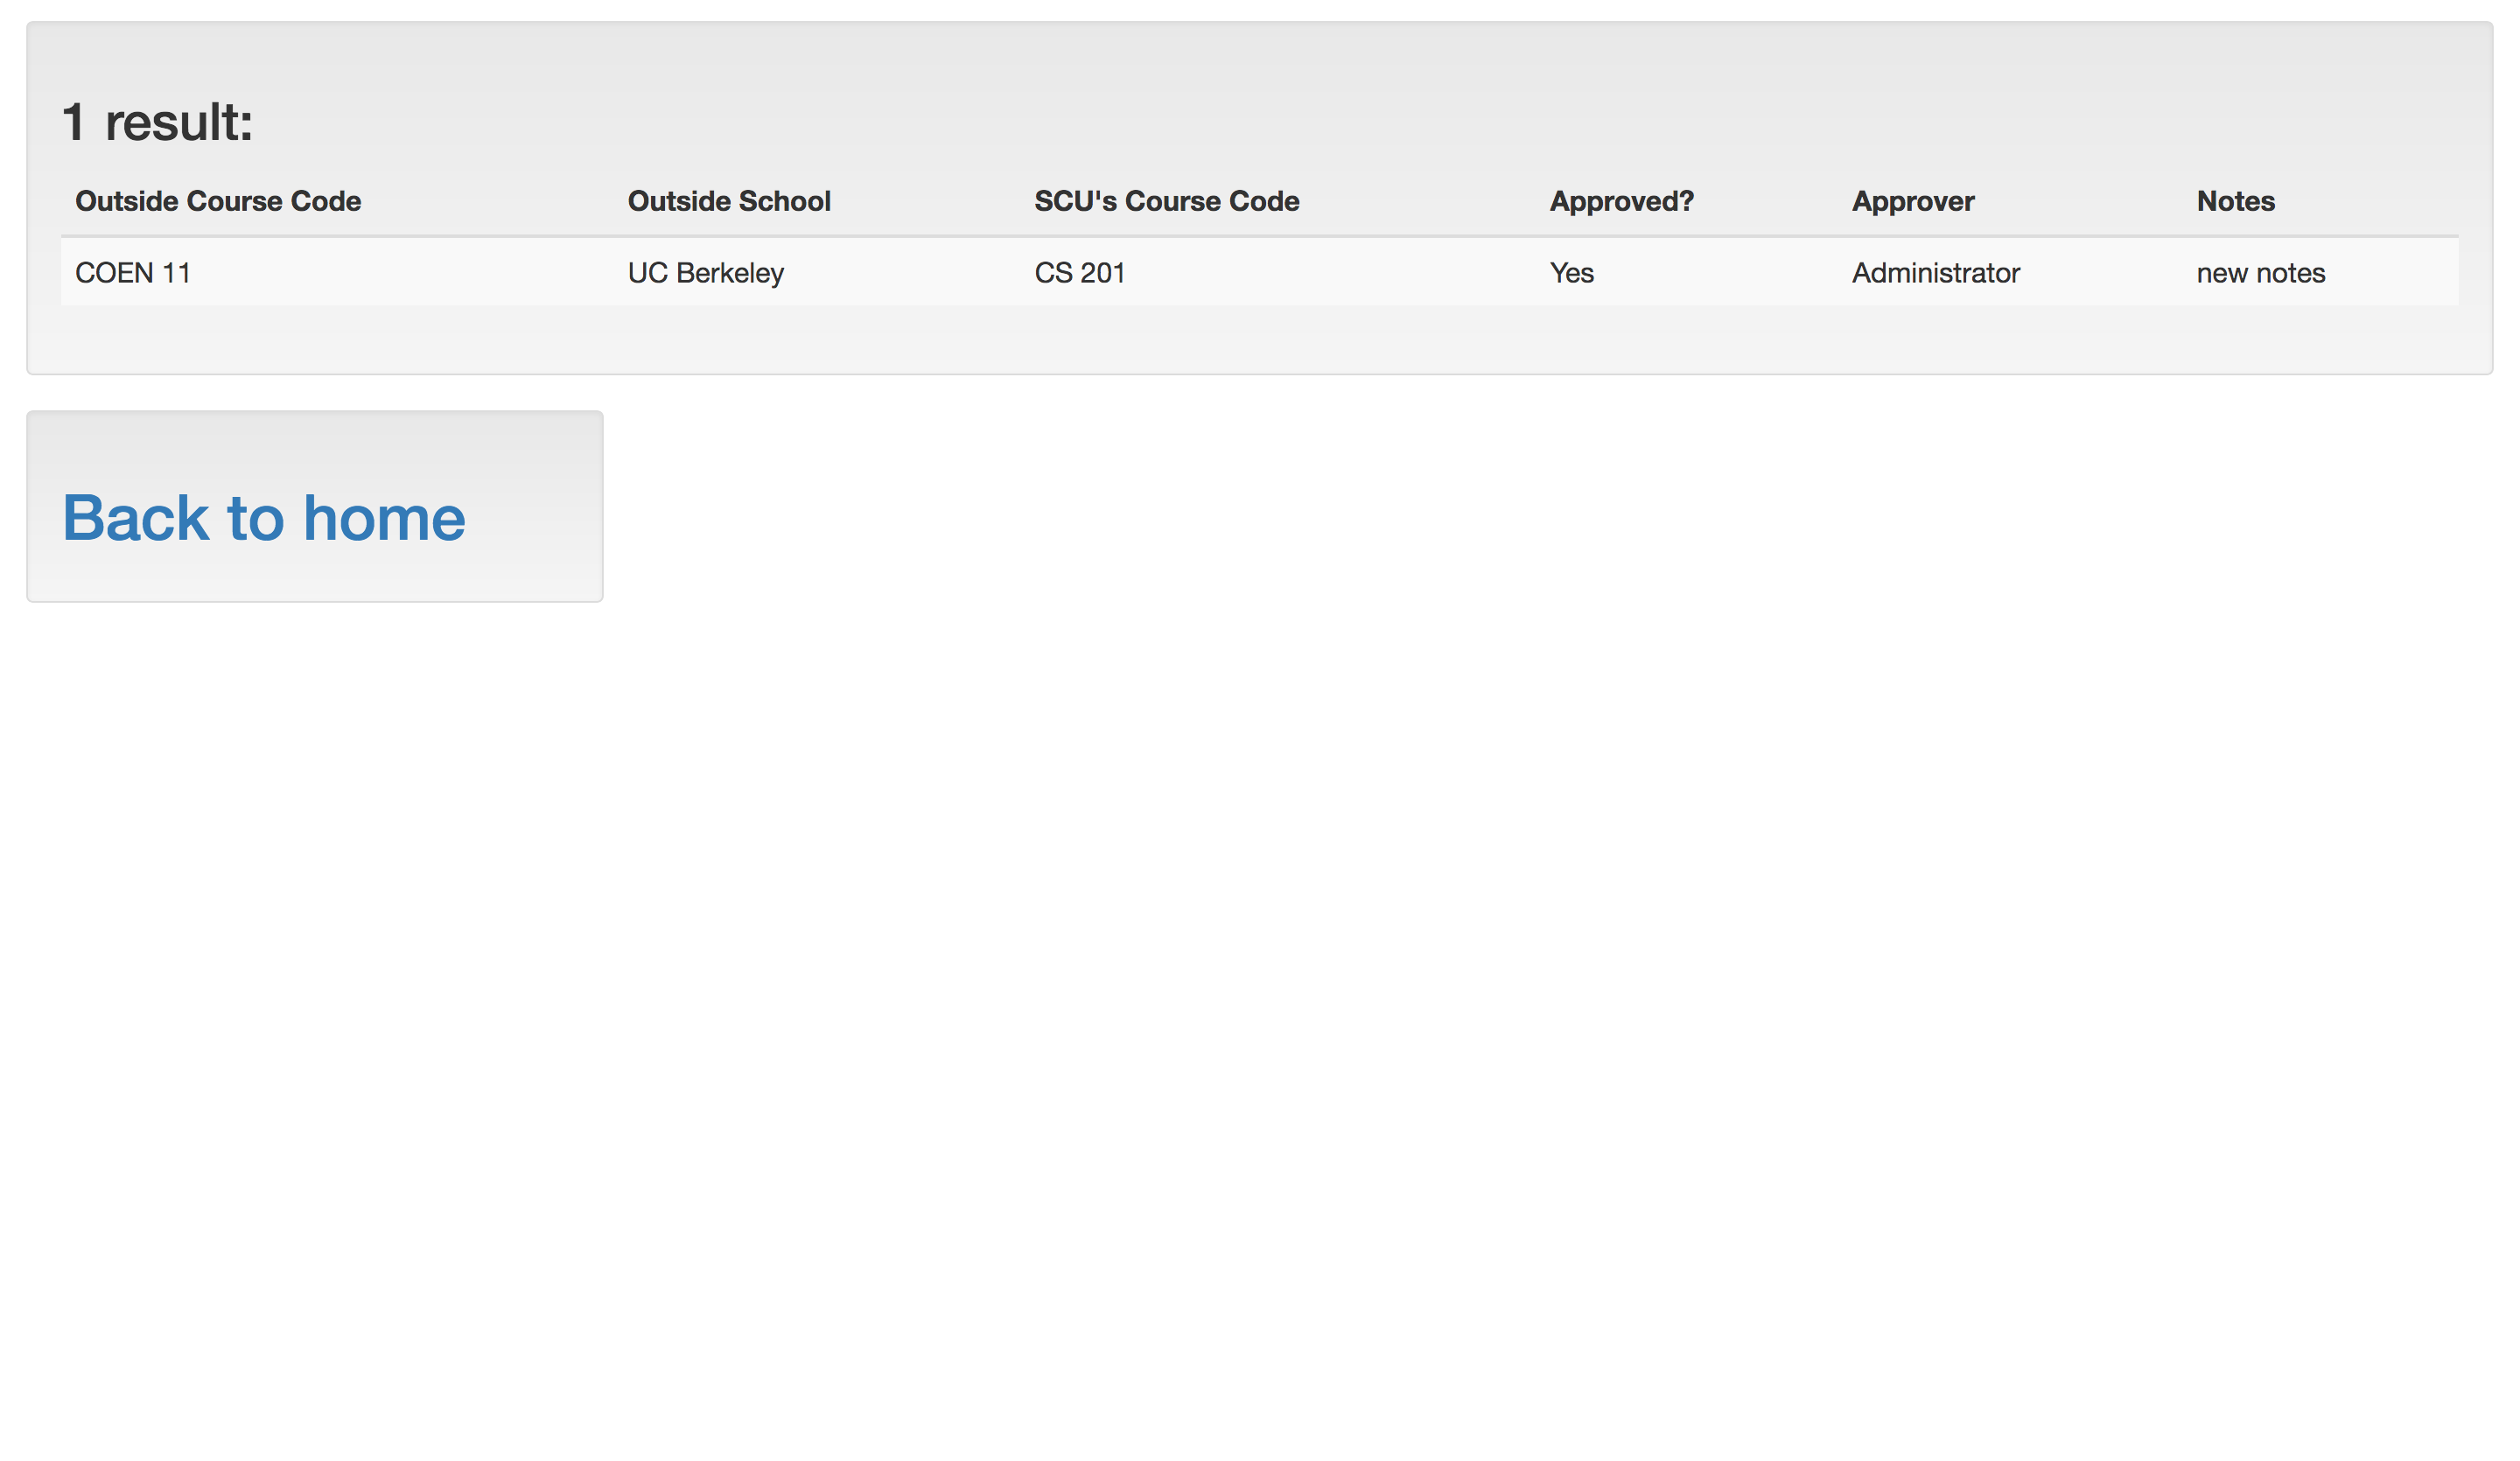
\includegraphics[width=15cm]{detailedview}
\centering
\caption{Detailed view}
\label{fig:detailedview}
\end{figure}

\section{Faculty Functionality}
\par Each faculty user has the ability to create course equivalencies, and later
modify or delete those equivalencies. Each faculty user may only modify or
delete equivalencies that he/she has created.

\par Before creating, modifying, or deleting an equivalency, a faculty user must log in.
To do this, click on the ``Faculty login'' button on the home page. This will
open an area that prompts the user to enter his/her login credentials, as shown
in \cref{fig:login}. Enter the login credentials provided to you by your network
administrator into the ``username'' and ``password'' fields, and then click submit.
If you entered the credentials correctly, the page will refresh, and you will be
successfully logged in, as shown in \cref{fig:loggedin}.

\begin{figure}[h]
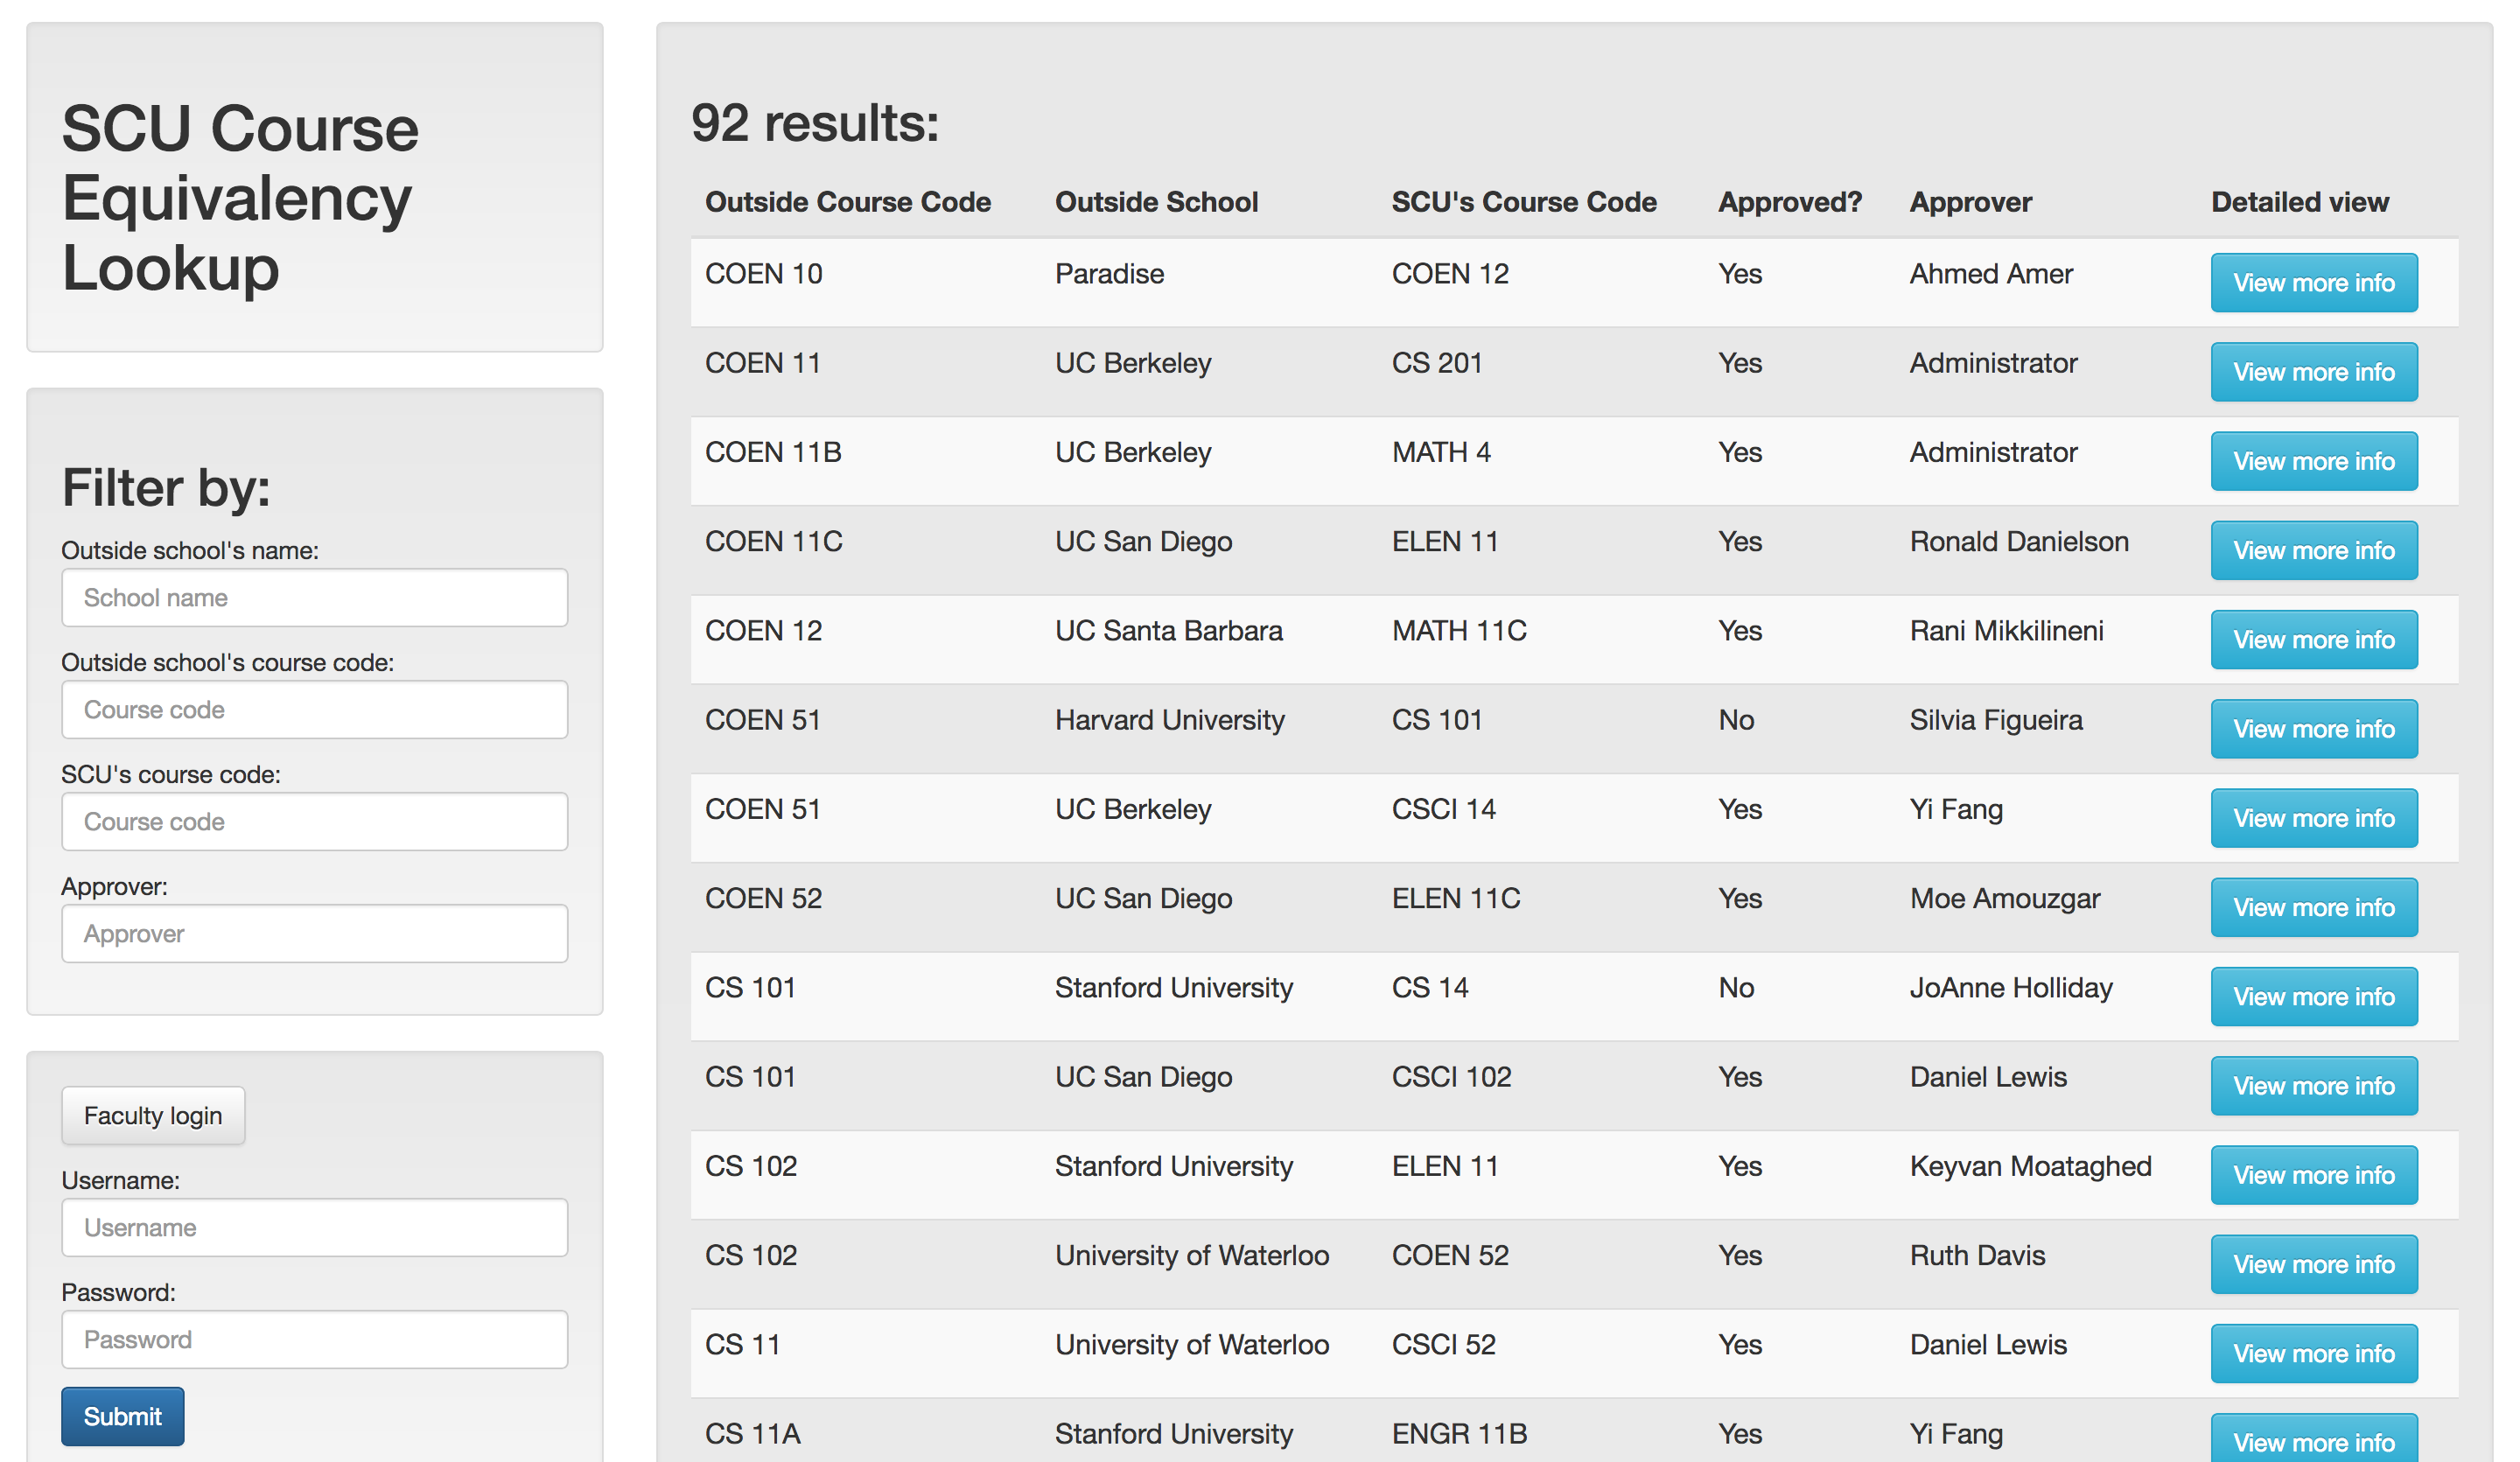
\includegraphics[width=15cm]{login}
\centering
\caption{Log in prompt}
\label{fig:login}
\end{figure}

\begin{figure}[h]
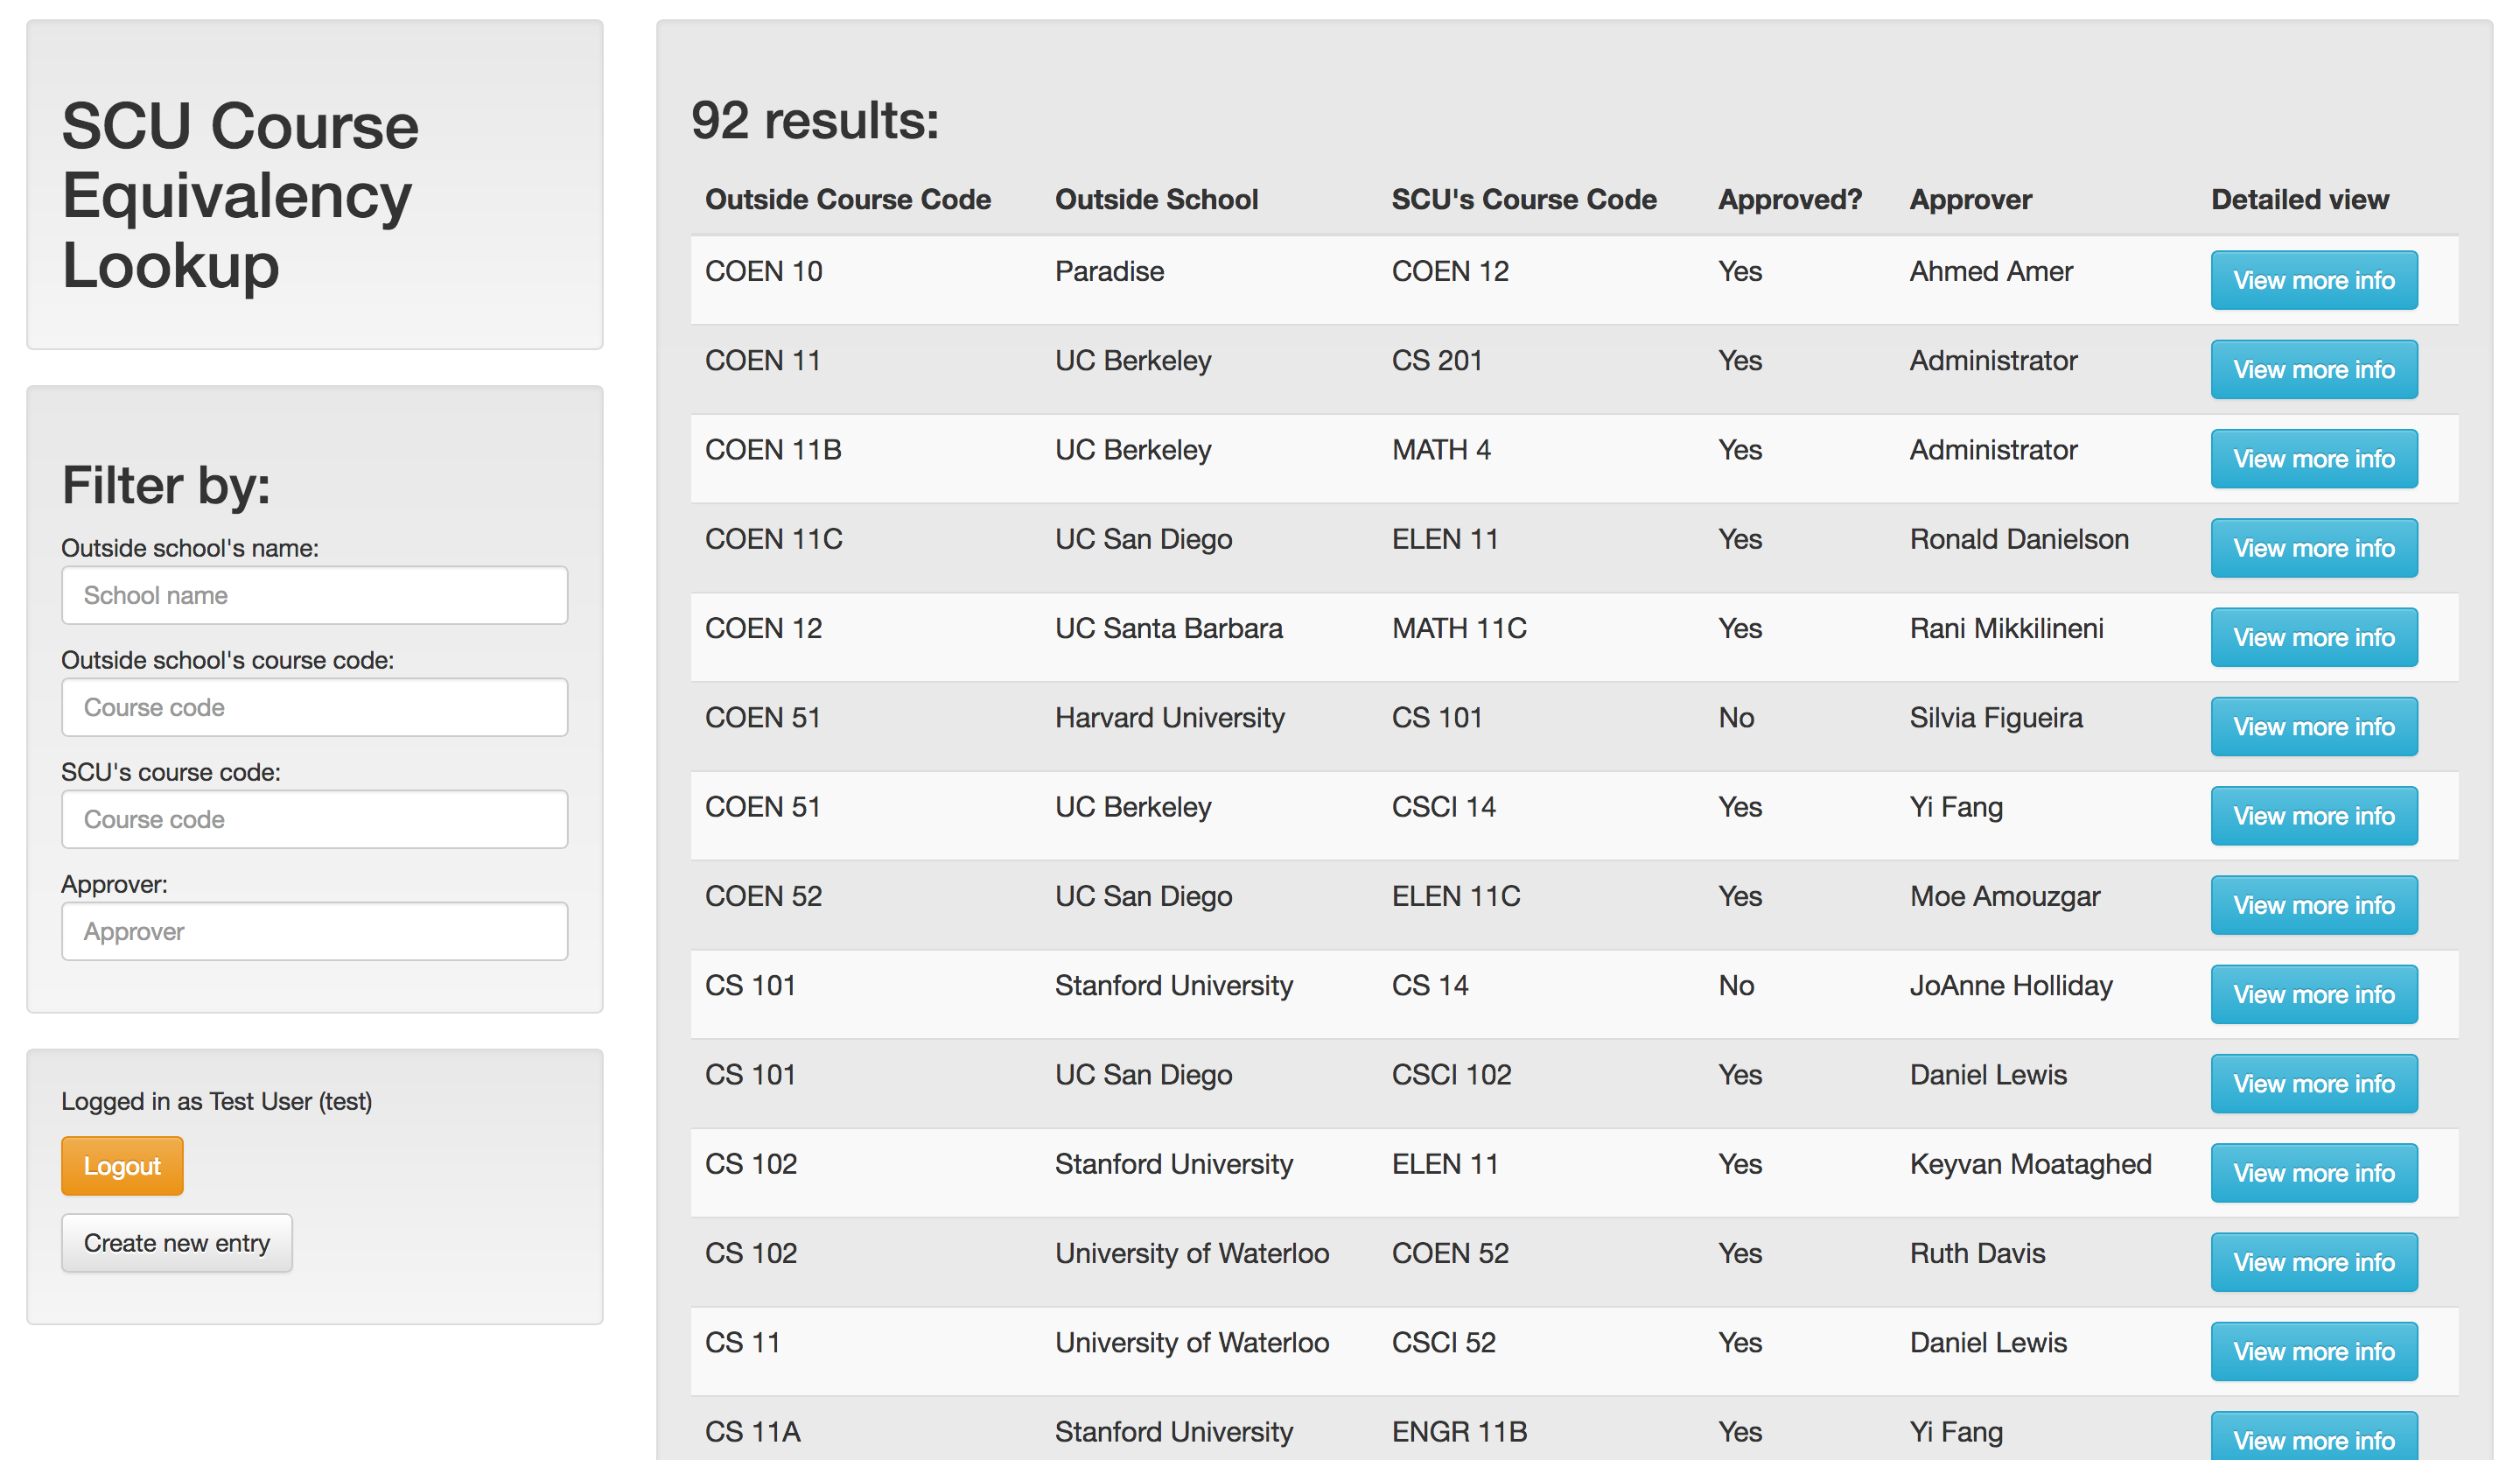
\includegraphics[width=15cm]{loggedin}
\centering
\caption{Logged in user}
\label{fig:loggedin}
\end{figure}

\par After logging in, you may create an equivalency, and you may also modify or
delete any equivalency which you have created. To create an equivalency, click
on the ``Create new entry'' button below the orange ``Logout'' button on the left
side of the screen. This will open an area that prompts you to enter various
fields required for the equivalency. See \cref{fig:addequivalency}. To create an equivalency, you
must fill out the fields ``Outside school's course code'',
``Outside school's name'', ``SCU's course code'', and ``Approved?''.
The ``Notes'' field is optional. Once you have filled out all of the required
fields, you may click the ``Submit'' button to create the equivalency. The page
will refresh, and your equivalency is now included in the list of equivalencies.

\begin{figure}[h]
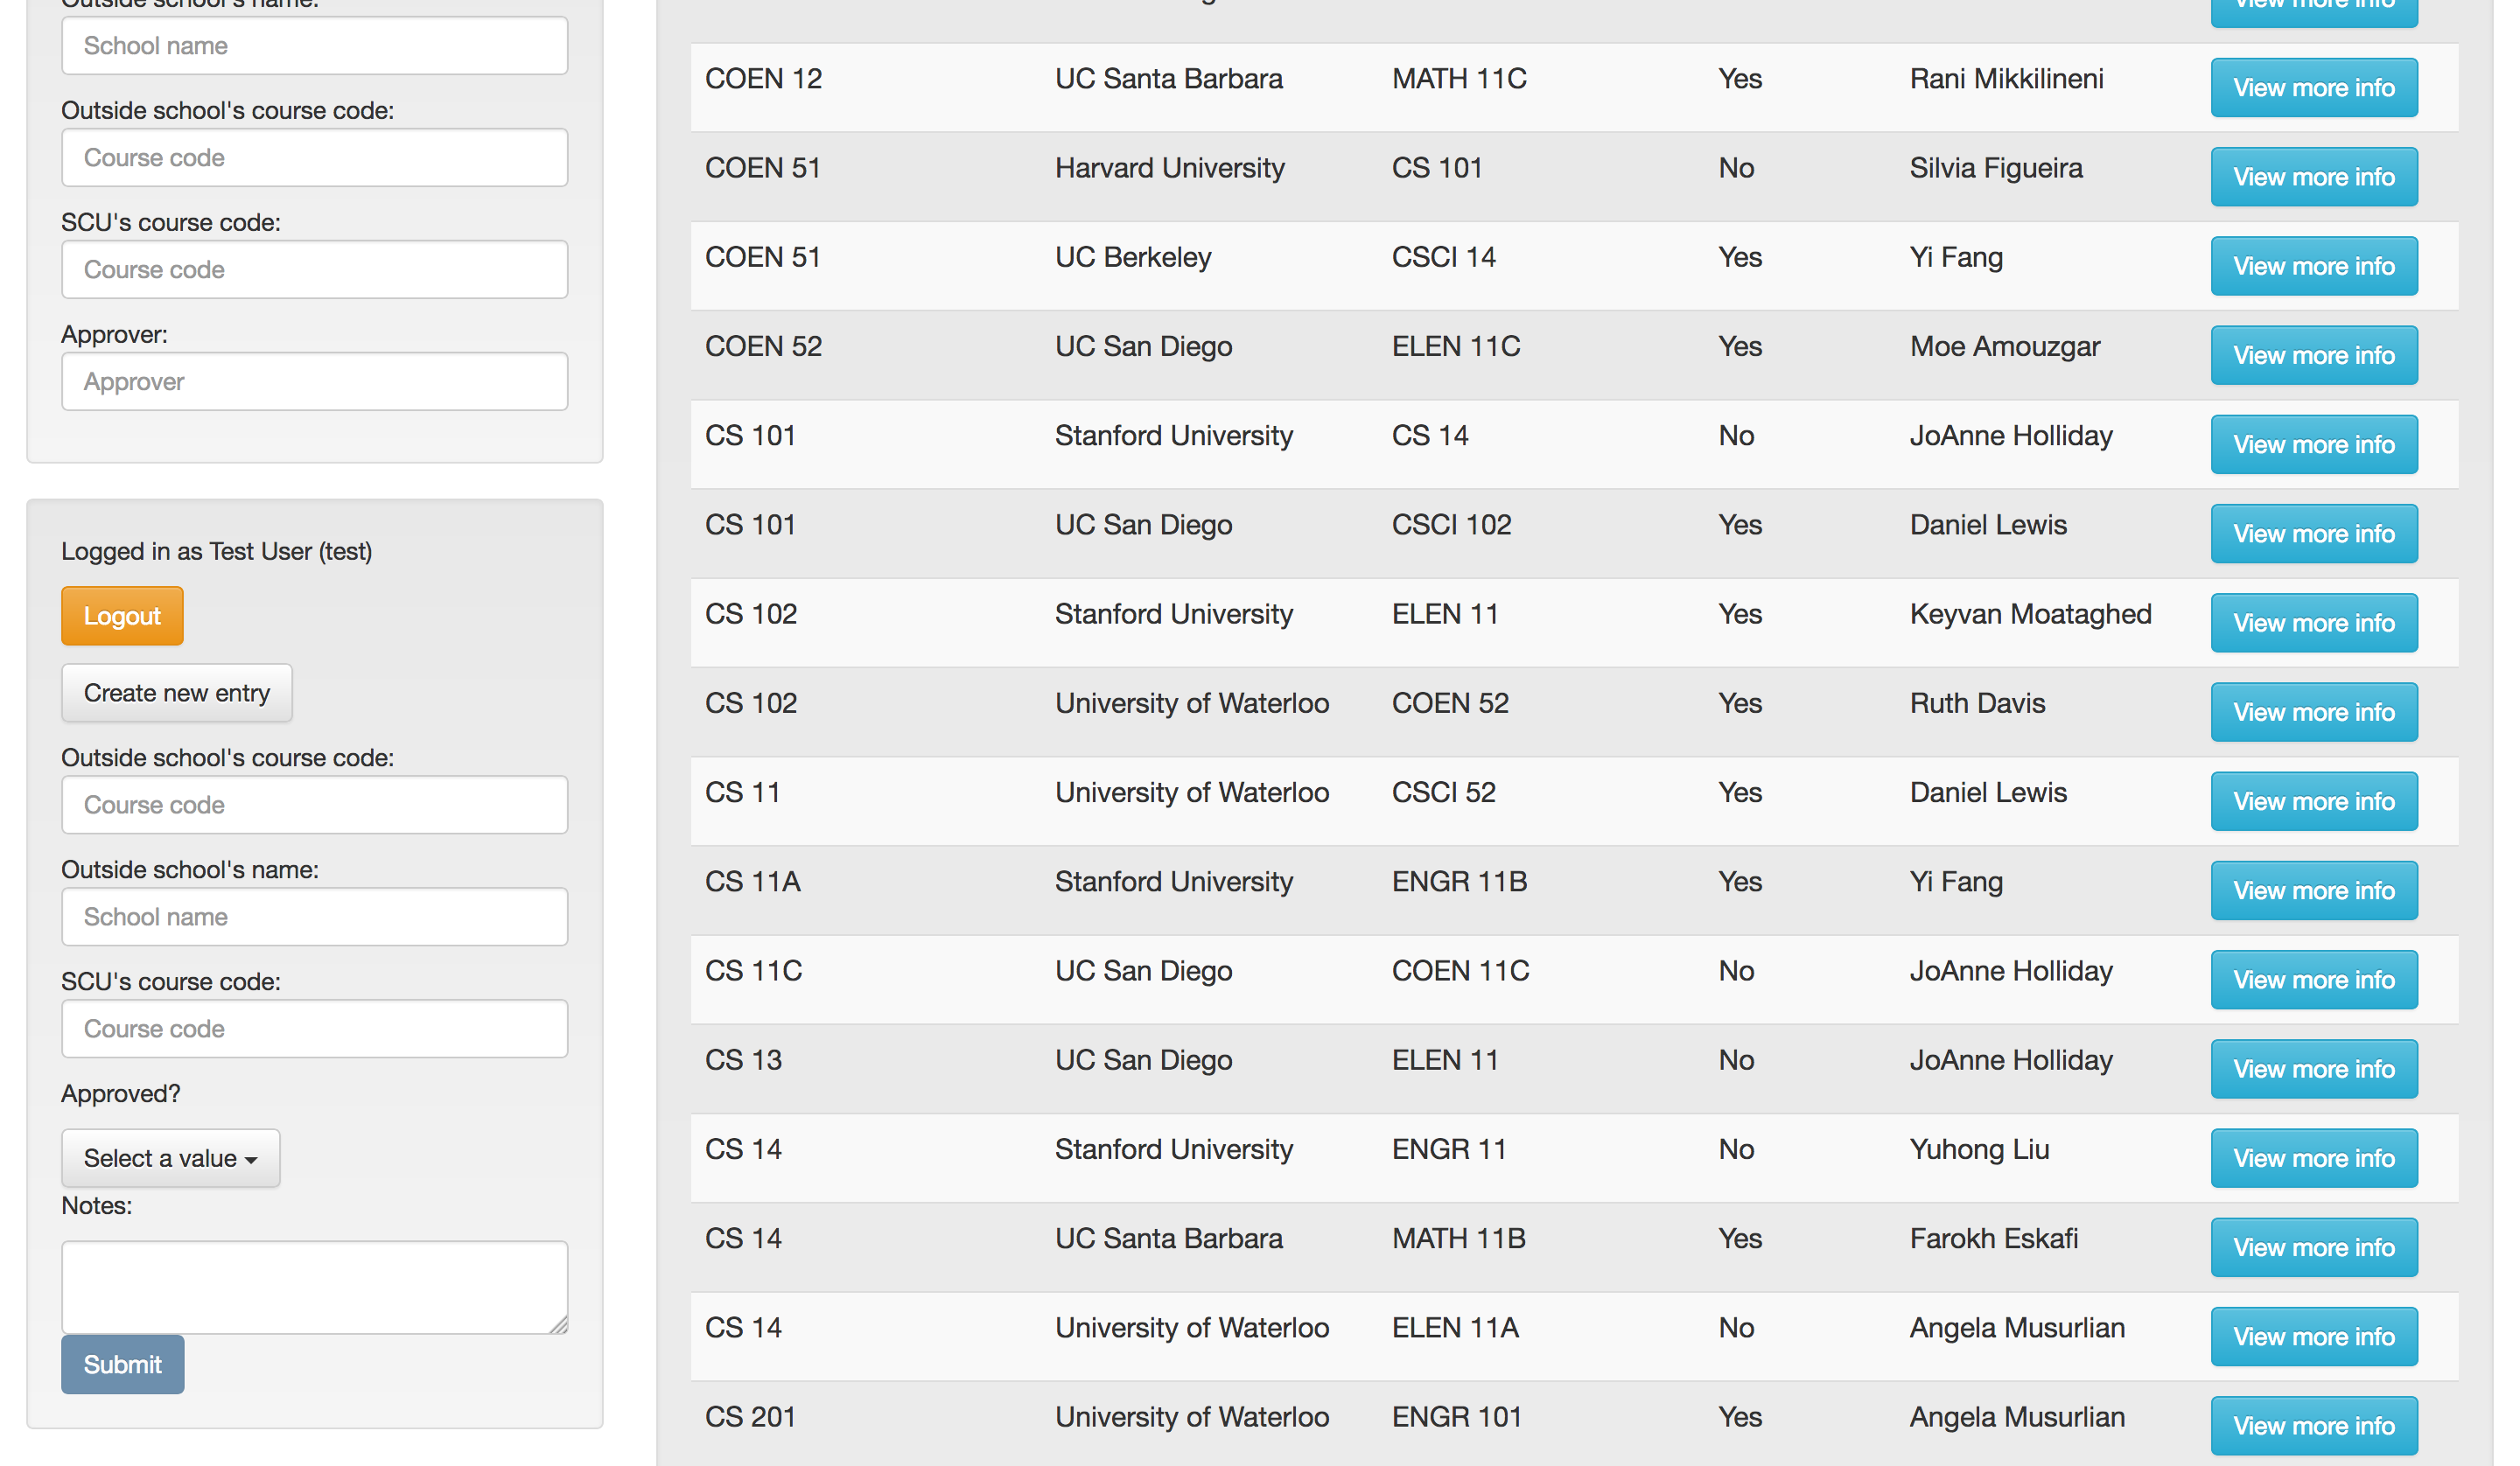
\includegraphics[width=15cm]{addequivalency}
\centering
\caption{Adding an equivalency}
\label{fig:addequivalency}
\end{figure}

\par You may also modify or delete any equivalency you have created. To do
this, click the ``View more info'' button on the equivalency that you wish to
modify or delete. This will redirect you to the detailed view shown in \cref{fig:modify}.
Note that this view is very similar to the one shown in \cref{fig:detailedview}, except when
logged in, the user is allowed to modify or delete his/her equivalency. To
modify the equivalency, change the fields as desired in the section headed by
``Modify this equivalency''. When you are satisfied with the changes you have
made, click the ``Submit'' button, and then click the ``Back to home'' link to
return to the home page. To delete the equivalency, simply click the red
``Delete'' button. The equivalency will be deleted, and you will be redirected
to the home page.

\begin{figure}[h]
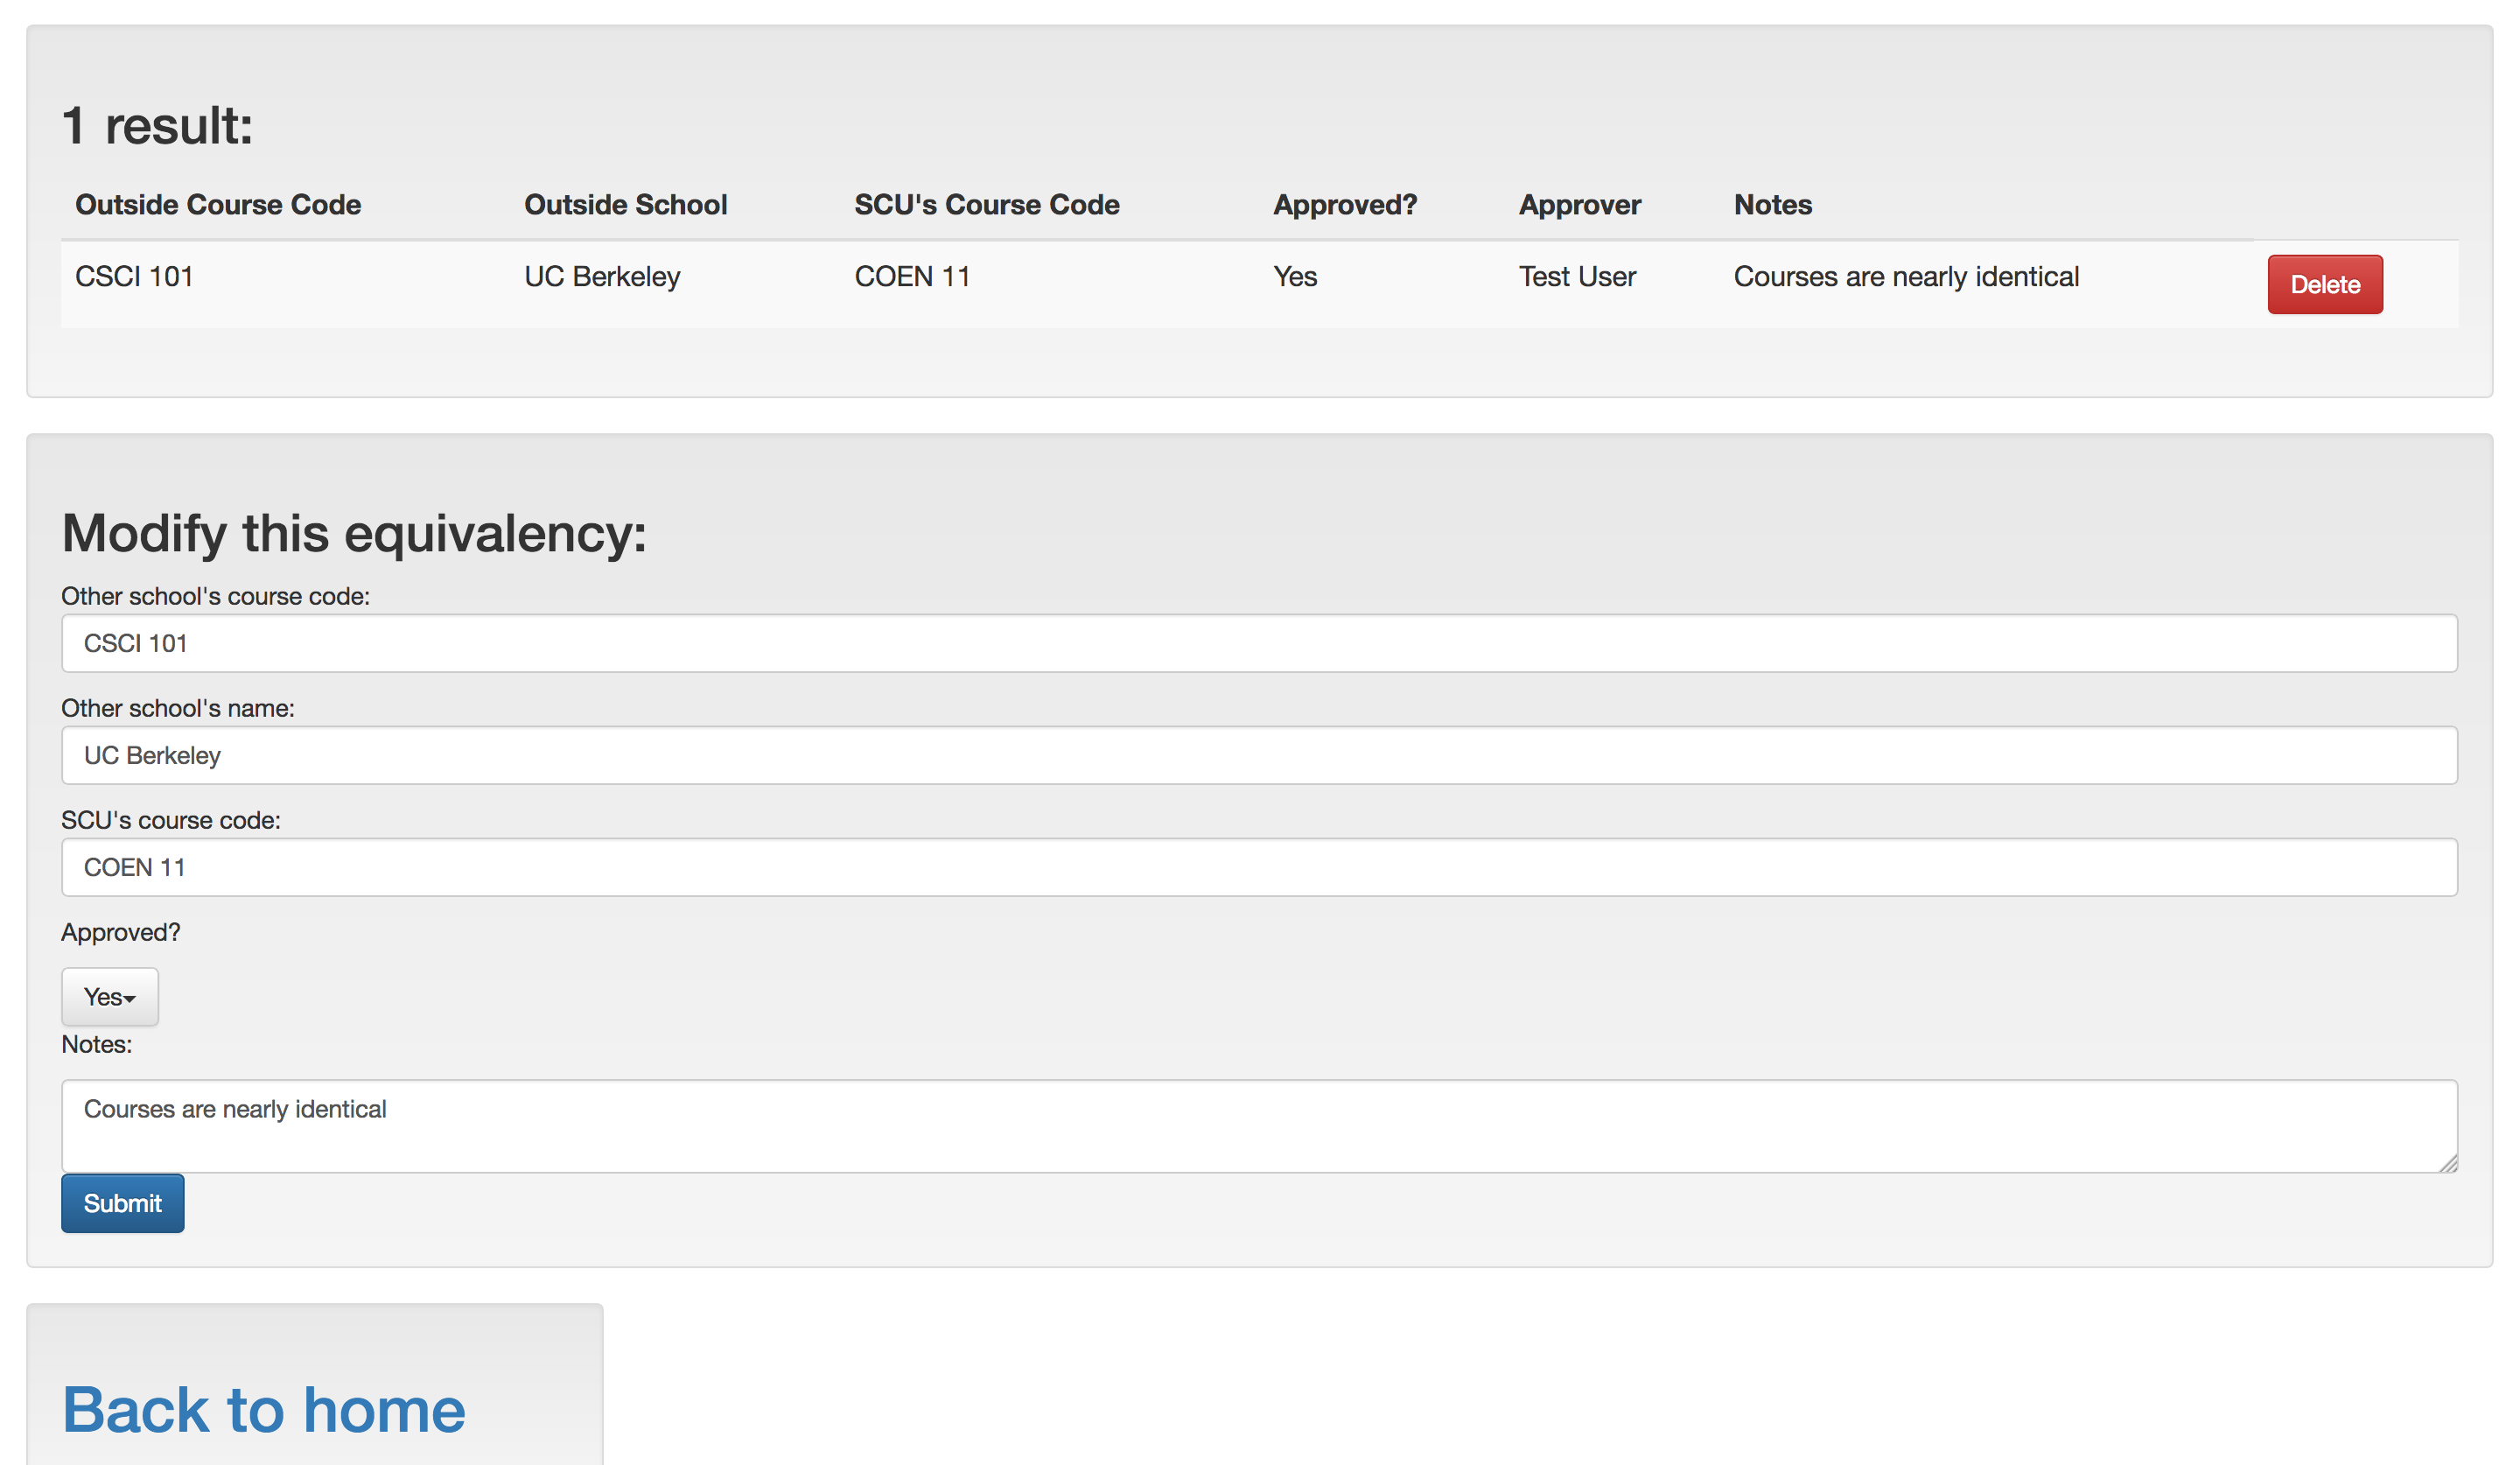
\includegraphics[width=15cm]{modify}
\centering
\caption{Modify or delete an equivalency}
\label{fig:modify}
\end{figure}

\par To log out, navigate to the home page and click the yellow ``Logout'' button.

\section{Administrator Functionality}
\par There exists a superuser for this system, whose username is ``admin'' and
real name within the system is ``Administrator''. The administrator may create
equivalencies, as well as modify and delete any other user's equivalencies.
When the administrator modifies another user's equivalency, the approver for
that equivalency will be changed to ``Administrator''.

\par Additionally, the administrator alone has the ability to create new faculty
users. To do so, first log in as the administrator. When you are logged in as
the administrator and are on the home page, there will be an additional button
available to you, labelled ``Create new faculty user''. See \cref{fig:admin}.

\begin{figure}[h]
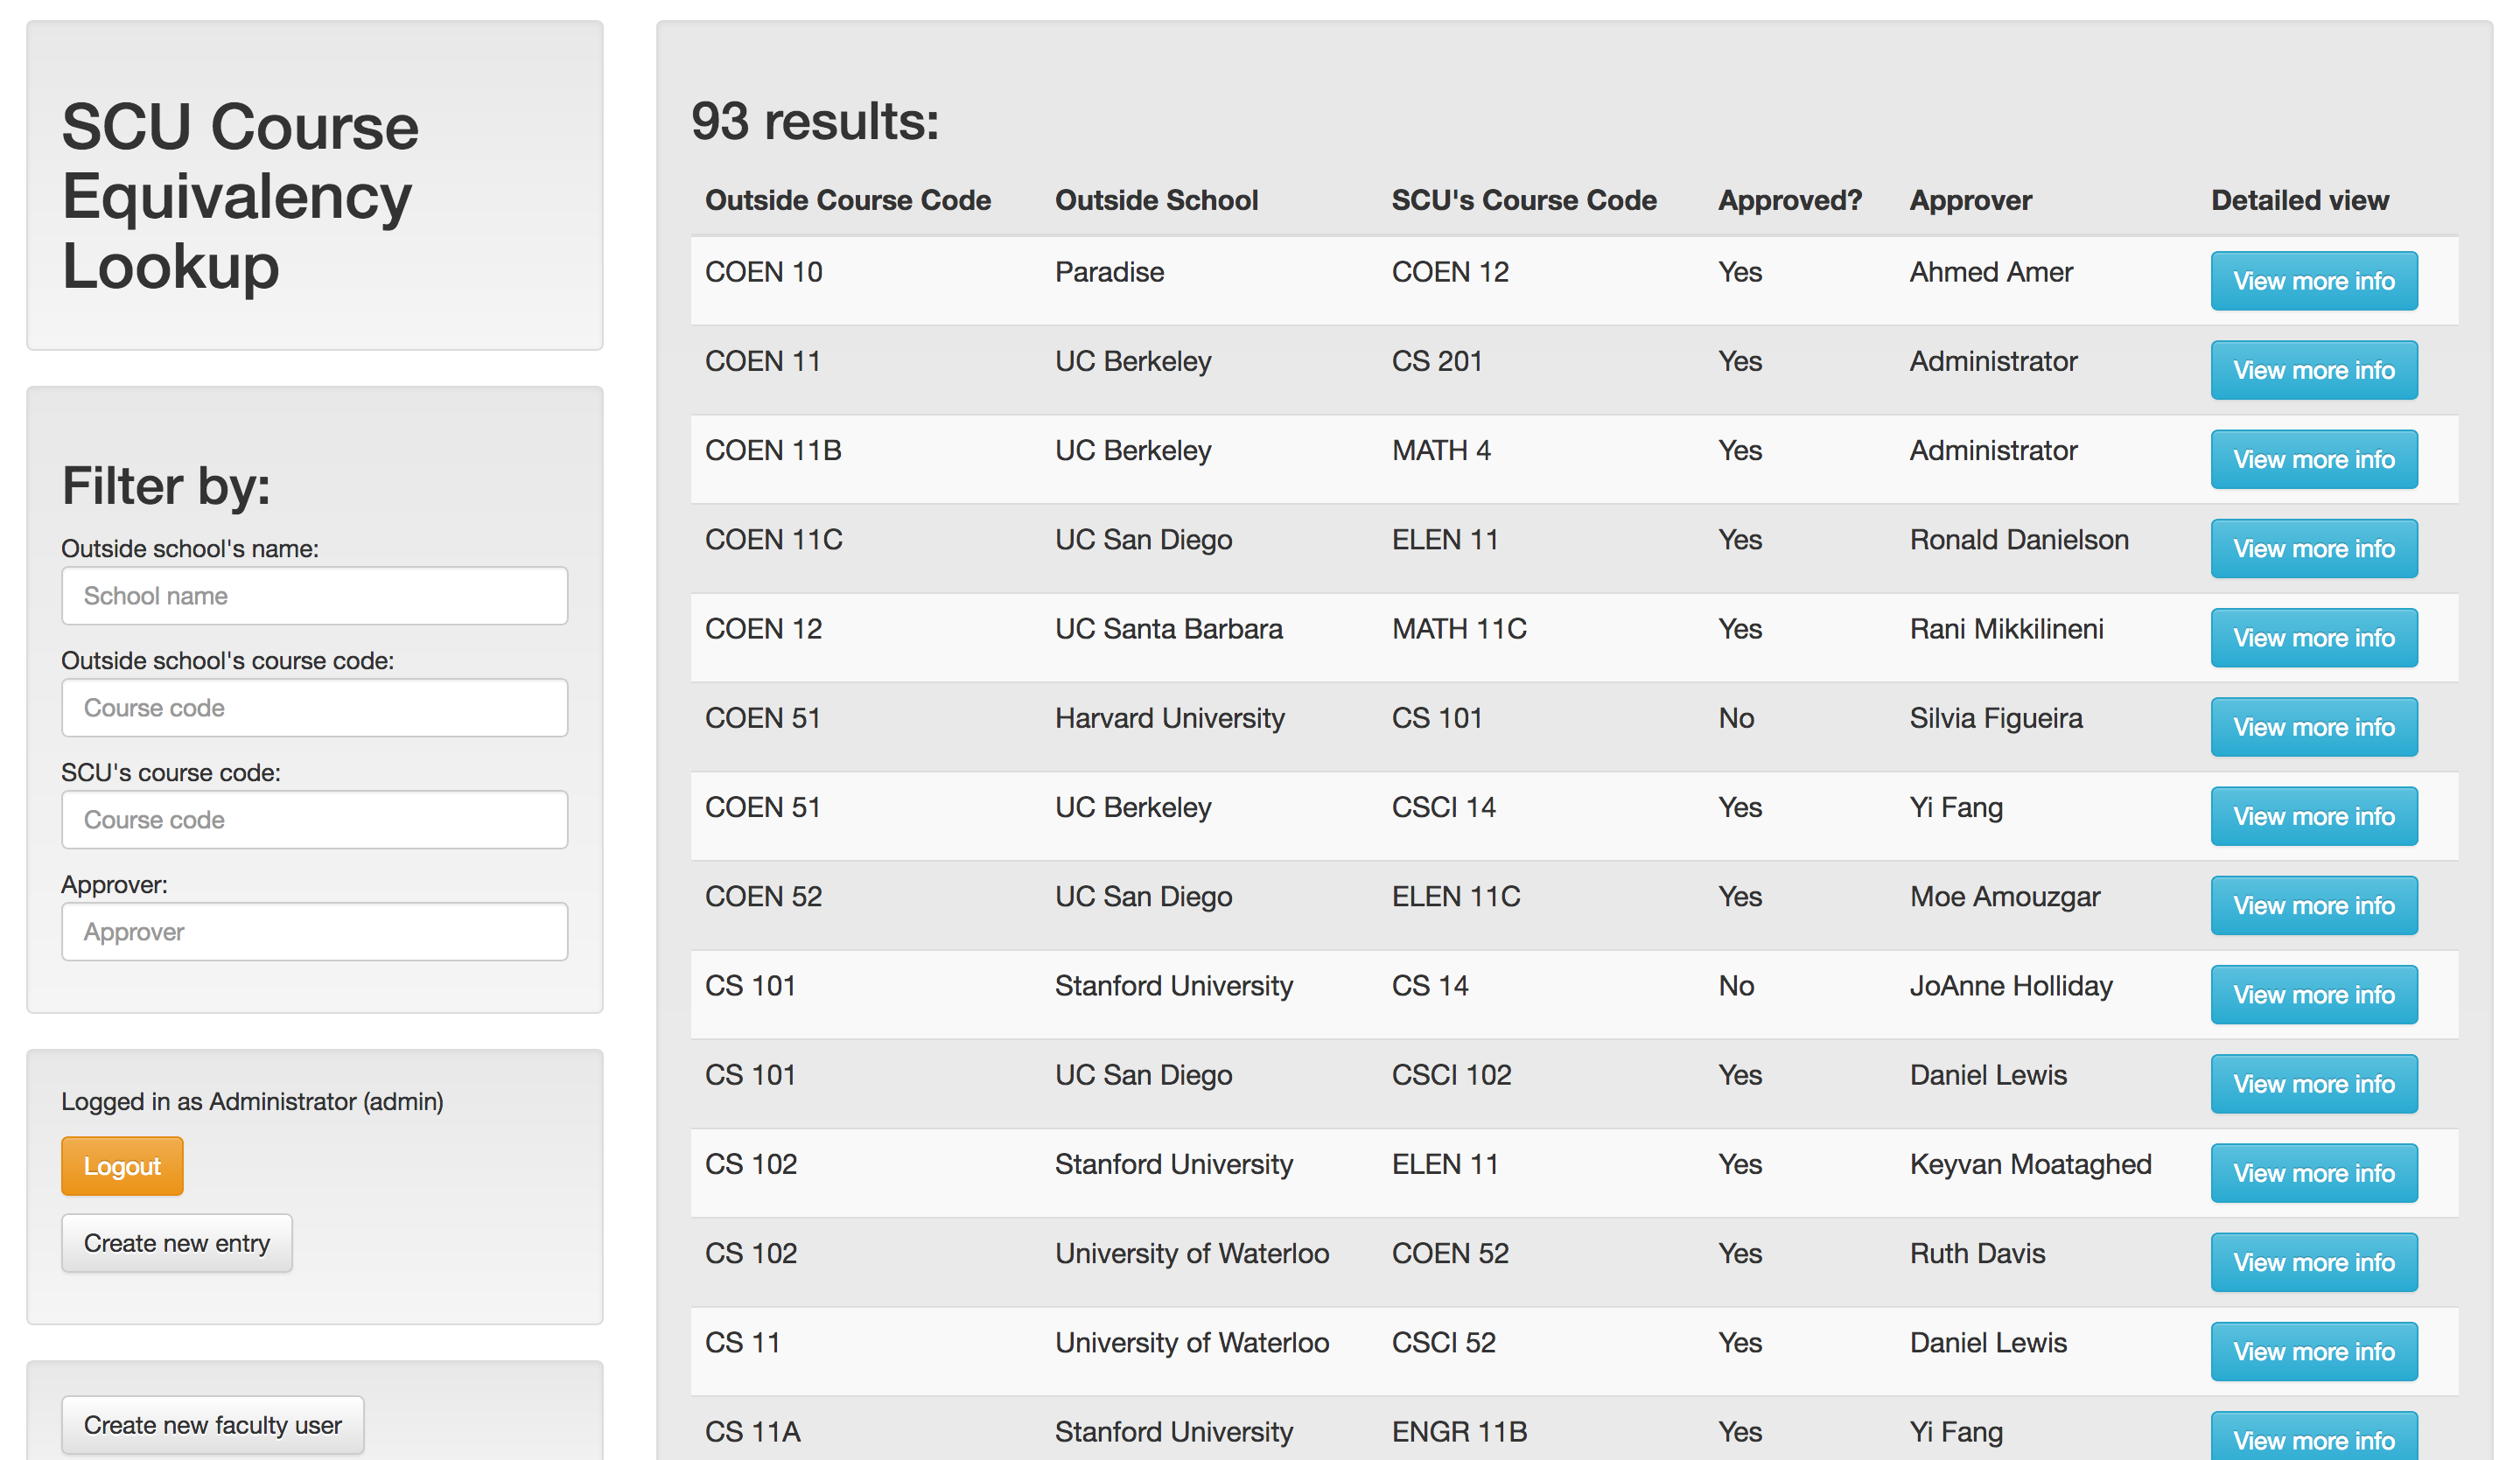
\includegraphics[width=15cm]{admin}
\centering
\caption{Admin home page}
\label{fig:admin}
\end{figure}

\par To create a new faculty user, click on the ``Create new faculty user''
button. This will open an area which prompts you to enter the username,
password, and real name of the new user. See \cref{fig:adduser}.

\begin{figure}[h]
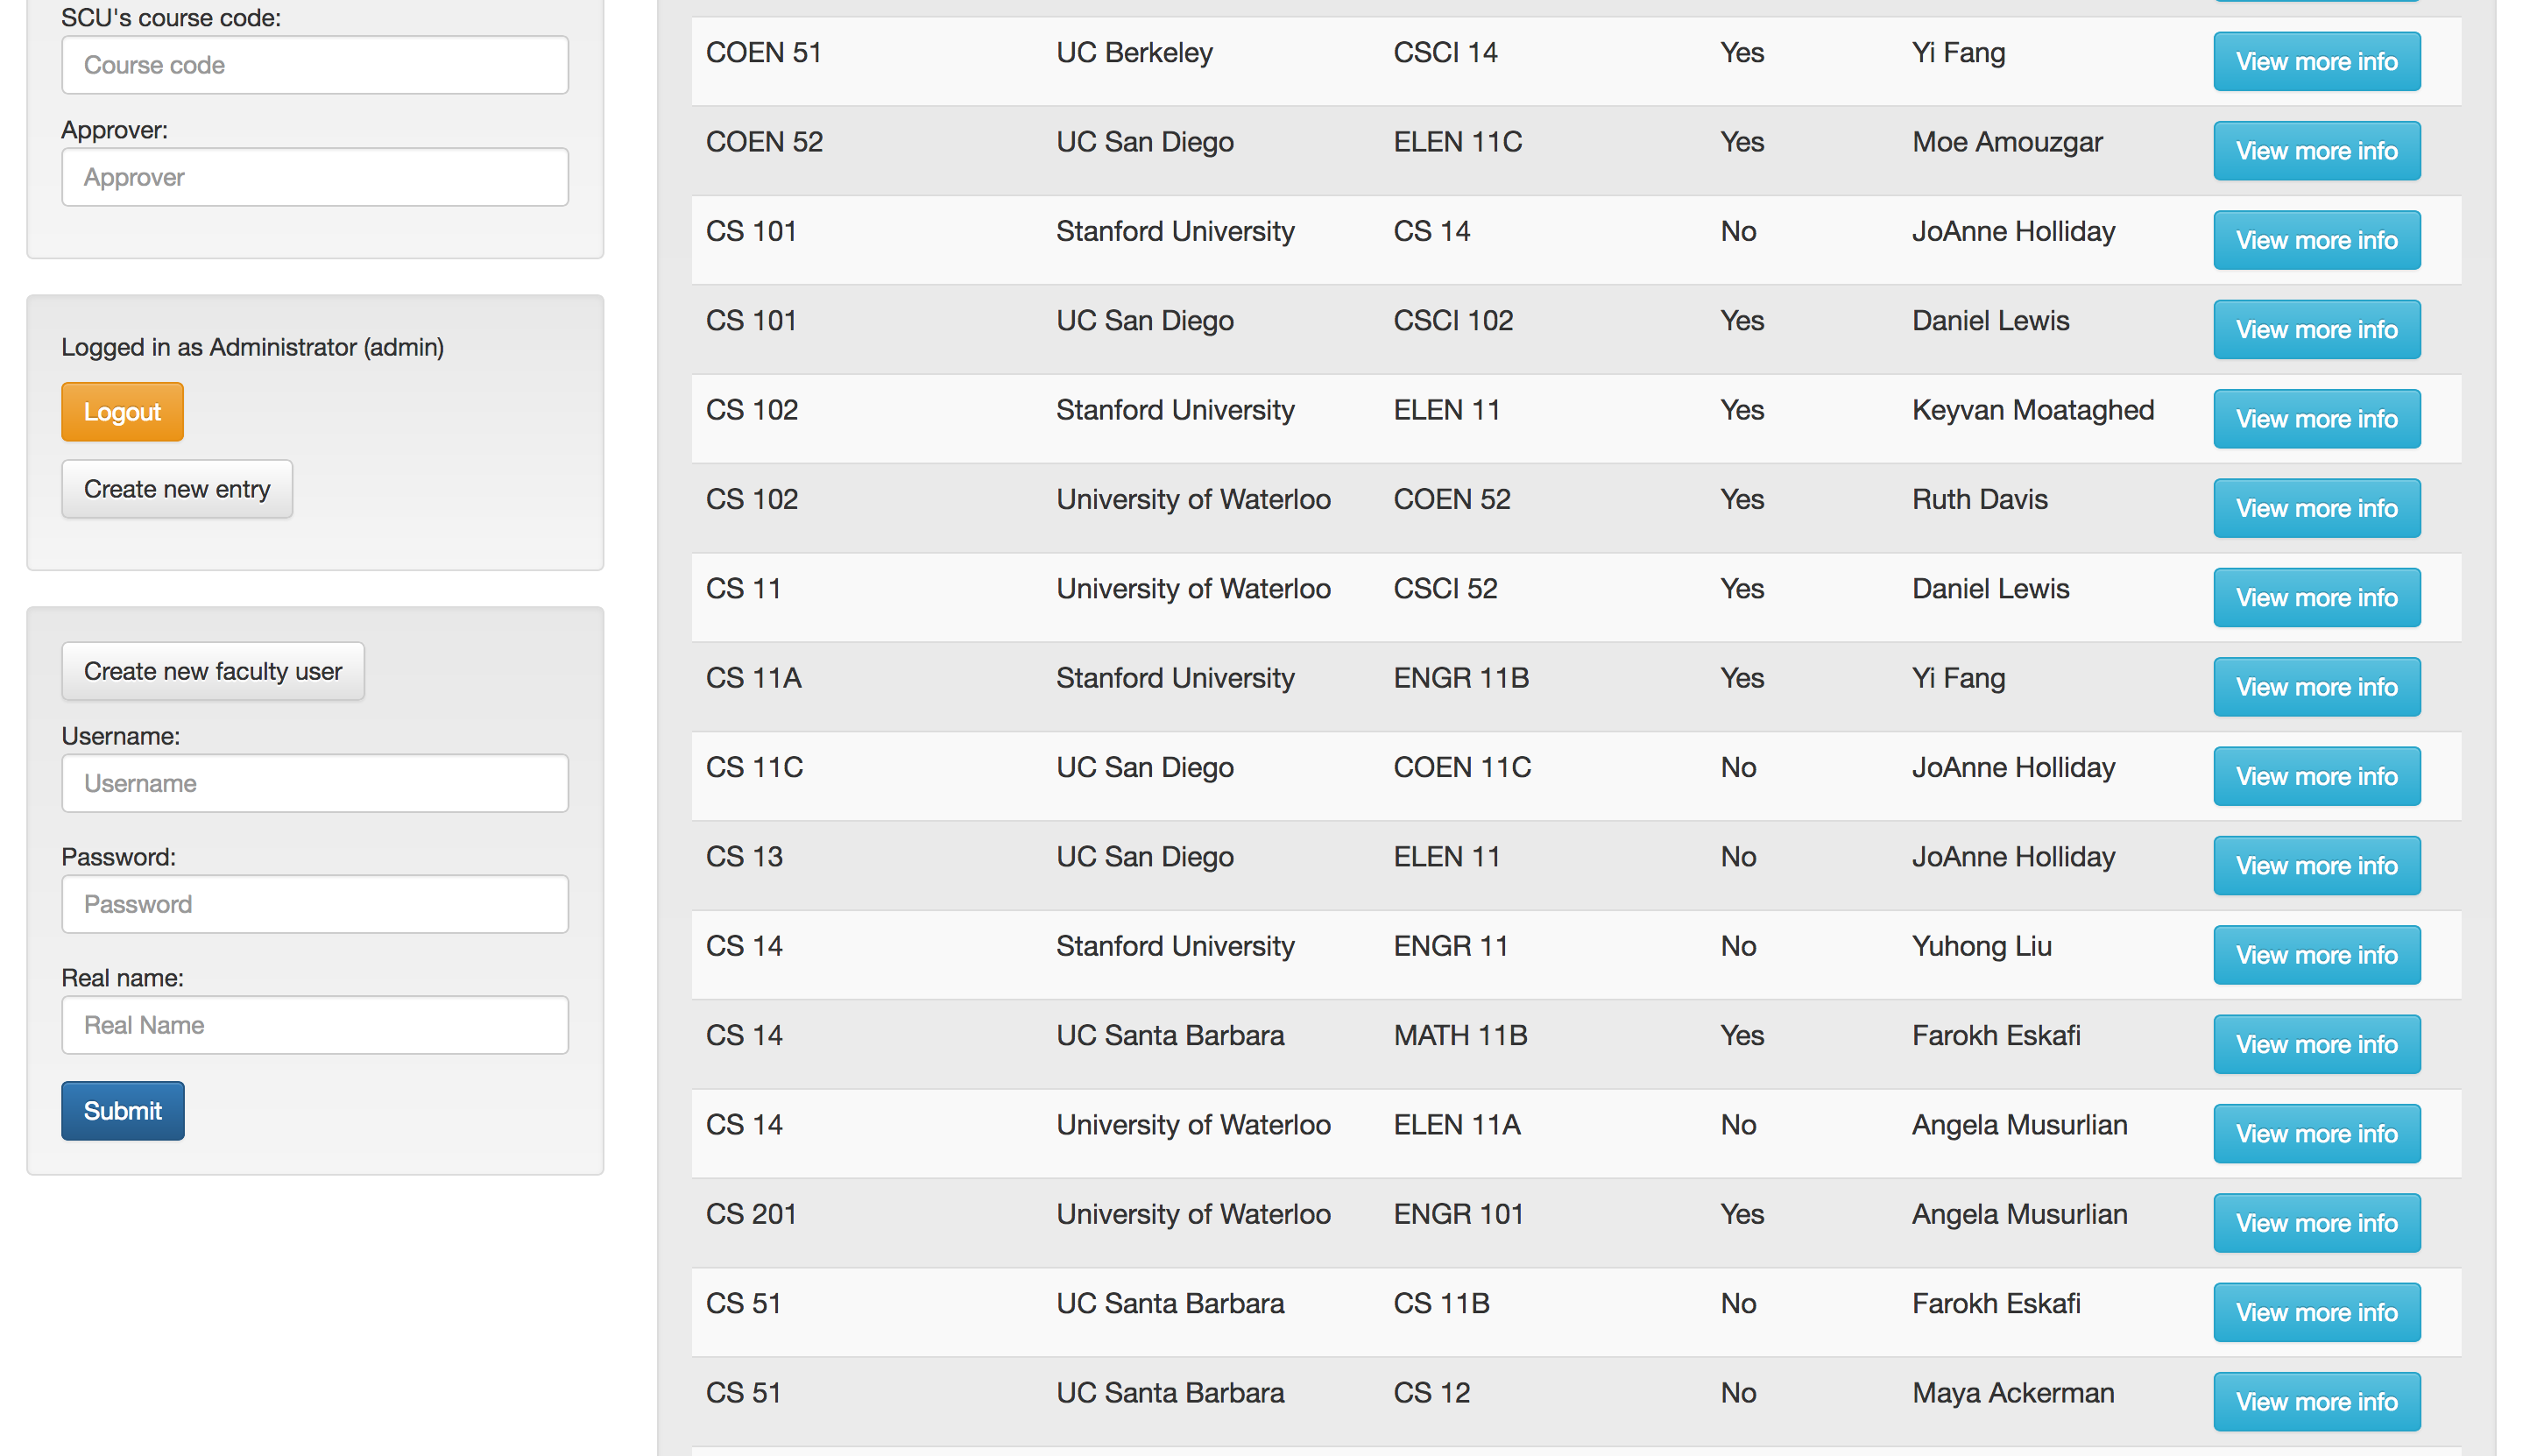
\includegraphics[width=15cm]{adduser}
\centering
\caption{Adding a new faculty user}
\label{fig:adduser}
\end{figure}

\par Enter the username, password, and real name of the new faculty user, and
click the ``Submit'' button once you have entered the information. If the user
already exists, a dialog box will open and notify you as such, and you must
choose a different username. Otherwise, the user will be added. To log in as
this user, you must log out as the administrator user, and then log in as the
new user, using the steps detailed in the ``Faculty functionality'' section.
\end{document}
